\documentclass[../PianoDiQualifica_v4.0.0.tex]{subfiles}

\begin{document}

\section{Specifica dei test}
\kpanic\ ha strutturato alcuni test atti a verificare che il software prodotto sia efficace. Questi test sono basati sulle tecniche di verifica dinamica introdotte nel documento \normediprogettov. Il team ha deciso di produrre alcune tabelle per facilitare la consultazione ed il tracciamento di tutte le attività eseguite e dei risultati ottenuti.\\ Nello specifico sono stati presi in considerazione quattro tipologie di test, rispettivamente:
\begin{itemize}
	\item \textbf{Test di unità [TU]:} cerca di verificare la più piccola parte di lavoro prodotta da un programmatore che funzioni in modo autonomo, la quale può essere una funzione o una classe;
	\item \textbf{Test di integrazione [TI]:} cerca di verificare un insieme di unità, che prendono il nome di componenti di sistema, secondo diversi approcci quali, tra i più famosi:
	\begin{itemize}
		\item Top-down;
		\item Bottom-up;
		\item Umbrella, un ibrido dei due precedenti.
	\end{itemize}
	\item \textbf{Test di sistema [TS]:} cerca di verificare che il comportamento e il funzionamento di una o più componenti software siano corretti secondo i propri requisiti;

	\item \textbf{Test di non regression [TNR]:} sono svolti con l’obiettivo di verificare che, avendo apportato una modifica ad una parte del codice, non risulti compromessa la correttezza di altre funzioni collegate.

	\item \textbf{Test di validazione [TV]:} chiamati anche test di accettazione, cerca di verificare che il lavoro prodotto soddisfi quanto richiesto dal proponente. Nella pratica, attraverso delle funzioni, si cerca di simulare il comportamento generale dell'applicativo e dell'utente che interagisce con esso.
\end{itemize}

	\newpage
	\subsection{Test di unità}
	I test di unità saranno descritti nel modo seguente:
	\begin{center}
		\textbf{TU[IdTest]}
	\end{center}
	dove:
	\begin{itemize}
		\item \textbf{IdComponente} rappresenta il codice identificativo crescente dell'unità considerata.
	\end{itemize}

	\begin{longtable}[c] { >{\centering\arraybackslash}p{2cm} p{9cm} >{\centering\arraybackslash}p{4cm}}
		\toprule
		\centerline{\textbf{ID test}} & \centerline{\textbf{Descrizione}} & \centerline{\textbf{Stato}} \\
			\midrule
			TU0 & Verificare che il metodo \textbf{addAdmin} aggiunga nella lista degli admin l'oggetto passato come parametro & Implementato \\
			\addlinespace[0.3em]
			\midrule
			\addlinespace[0.3em]
			TU1 & Verificare che il metodo \textbf{updateAdmin} modifichi correttamente i dati dell'admin contenuti nel Database con quelli contenuti all'interno dell'oggetto passato come parametro & Implementato \\
			\addlinespace[0.3em]
			\midrule
			\addlinespace[0.3em]
			TU2 & Verificare che il metodo \textbf{deleteAdmin} elimini correttamente l'admin che corrisponde all'oggetto passato come parametro all'interno del Database & Implementato \\
			\addlinespace[0.3em]
			\midrule
			\addlinespace[0.3em]
			TU3 & Verificare che il metodo \textbf{getAdmins} restituisca correttamente un array di oggetti contenenti tutti gli utenti che sono amministratori & Implementato \\
			\addlinespace[0.3em]
			\midrule
			\addlinespace[0.3em]
			TU4 & Verificare che il metodo \textbf{validateAdmin} restituisca esito di convalida (TRUE o FALSE) dell'oggetto di tipo JSON schema passato come parametro & Implementato \\
			\addlinespace[0.3em]
			\midrule
			\addlinespace[0.3em]
			TU5 & Verificare che il metodo \textbf{validateUpdate} restituisca esito di convalida (TRUE o FALSE)dell'oggetto di tipo JSON schema passato come parametro & Implementato \\
			\addlinespace[0.3em]
			\midrule
			\addlinespace[0.3em]
			TU6 & Verificare che il metodo \textbf{sendEmail} componga e spedisca una email all'indirizzo passato come parametro stringa solo nel caso in cui l'utente sia realmente presente all'interno del Database & Implementato \\
			\addlinespace[0.3em]
			\midrule
			\addlinespace[0.3em]
			TU7 & Verificare che il metodo \textbf{logout} termini correttamente la sessione dell'admin identificato dal token passato al metodo come parametro stringa & Implementato \\
			\addlinespace[0.3em]
			\midrule
			\addlinespace[0.3em]
			TU8 & Verificare che il metodo \textbf{login} controlli correttamente la presenza nel Database dell'utente il cui username coincide con il primo parametro stringa passato al metodo e, nel caso questo primo controllo vada a buon fine, procede verificando che la password che corrisponde allo username appena individuato coincida con quella passata come secondo parametro sotto forma di stringa. Se uno dei due controlli non va a buon fine viene generato un errore & Implementato \\
			\addlinespace[0.3em]
			\midrule
			\addlinespace[0.3em]
			TU9 & Verificare che il metodo \textbf{verifyLogin} controlli correttamente che il token passato come parametro stringa coincida con quello presente nel Database collegato all'utente della sessione corrente e, nel caso il controllo vada a buon fine, torna TRUE, altrimenti torna FALSE & Implementato \\
			\addlinespace[0.3em]
			\midrule
			\addlinespace[0.3em]
			TU10 & Verificare che il metodo \textbf{validateAuth} controlli correttamente che l'oggetto passato come parametro sia un JSON schema valido ritornando TRUE, FALSE altrimenti & Implementato \\
			\addlinespace[0.3em]
			\midrule
			\addlinespace[0.3em]
			TU11 & Verificare che il metodo \textbf{passwordRecoveryToken}, dopo aver verificato che il token passato come paramentro sia corretto, permetta di modificare la password dell'amministratore &Implementato \\
			\addlinespace[0.3em]
			\midrule
			\addlinespace[0.3em]
			TU12 & Verificare che il metodo \textbf{getFirms} restituisca correttamente un array di oggetti di tipo Firm contenente tutte le aziende all'interno del Database & Implementato \\
			\addlinespace[0.3em]
			\midrule
			\addlinespace[0.3em]
			TU13 & Verificare che il metodo \textbf{updateFirm} modifichi correttamente i campi dati dell'oggetto di tipo Firm presente nel Database in base ai campi dati presenti all'interno dell'oggetto Firm passato come parametro il cui ID corrisponde a quello dell'oggetto presente nel Database & Implementato \\
			\addlinespace[0.3em]
			\midrule
			\addlinespace[0.3em]
			TU14 & Verificare che il metodo \textbf{getGuestConversation} ritorni correttamente un array di oggetti di tipo Conversation che rappresentano le conversazioni effettuate dall'utente passato come oggetto e che afferisce all'azienda passata come parametro Firm & Implementato \\
			\addlinespace[0.3em]
			\midrule
			\addlinespace[0.3em]
			TU15 & Verificare che il metodo \textbf{existFirm} ritorni correttamente il booleano TRUE se verifica la presenza dell'azienda con il nome che coincide a quello passato come parametro string all'interno del Database o FALSE, altrimenti & Implementato \\
			\addlinespace[0.3em]
			\midrule
			\addlinespace[0.3em]
			TU16 & Verificare che il metodo \textbf{existGuest} ritorni correttamente il booleano TRUE se verifica la presenza dell'ospite con il nome che coincide a quello passato come parametro string all'interno del Database o FALSE, altrimenti & Implementato \\
			\addlinespace[0.3em]
			\midrule
			\addlinespace[0.3em]
			TU17 & Verificare che il metodo \textbf{validateGuest} restituisca esito di convalida (TRUE o FALSE) dell'oggetto di tipo JSON schema passato come parametro & Implementato \\
			\addlinespace[0.3em]
			\midrule
			\addlinespace[0.3em]
			TU18 & Verificare che il metodo \textbf{validateFirm} restituisca esito di convalida (TRUE o FALSE) dell'oggetto di tipo JSON schema passato come parametro & Implementato \\
			\addlinespace[0.3em]
			\midrule
			\addlinespace[0.3em]
			TU19 & Verificare che il metodo \textbf{addToDefault} aggiunga correttamente un interlocutore alla lista degli interlocutori di default presente nel nostro Database & Implementato \\
			\addlinespace[0.3em]
			\midrule
			\addlinespace[0.3em]
			TU20 & Verificare che il metodo \textbf{refreshInterlocutor} registri correttamente all'interno del Database tutti gli interlocutori presenti all'interno del team Slack di zero12 & Implementato \\
			\addlinespace[0.3em]
			\midrule
			\addlinespace[0.3em]
			TU21 & Verificare che il metodo \textbf{removeToDefault} rimuova correttamente un interlocutore dalla lista degli interlocutori di default presente all'interno del Database & Implementato \\
			\addlinespace[0.3em]
			\midrule
			\addlinespace[0.3em]
			TU22 & Verificare che il metodo \textbf{getInterlocutors} ritorni correttamente un array contenente oggetti di tipo Interlocutor, i quali corrispondono a tutti gli interlocutori presenti all'interno del team di zero12. & Implementato \\
			\addlinespace[0.3em]
			\midrule
			\addlinespace[0.3em]
			TU23 & Verificare che il metodo \textbf{getDefaultInterlocutors} ritorni correttamente un array contenente oggetti di tipo Interlocutor, i quali corrispondono ai soli interlocutori presenti all'interno della lista degli interlocutori di default di \prop\ & Implementato \\
			\addlinespace[0.3em]
			\midrule
			\addlinespace[0.3em]
			TU24 & Verificare che il metodo \textbf{validateInterlocutor} restituisca esito di convalida (TRUE o FALSE) dell'oggetto di tipo JSON schema passato come parametro & Implementato \\
			\addlinespace[0.3em]
			\midrule
			\addlinespace[0.3em]
			TU25 & Verificare che il metodo \textbf{sendMessageChannel} scriva correttamente un messaggio, il cui testo viene passato come parametro stringa al metodo, nel canale il cui nome viene anch'esso passato come parametro stringa. & Implementato \\
			\addlinespace[0.3em]
			\midrule
			\addlinespace[0.3em]
			TU26 & Verificare che il metodo \textbf{sendMessageGeneral} scriva correttamente un messaggio, il cui testo viene passato come parametro stringa al metodo, nel canale General & Implementato \\
			\addlinespace[0.3em]
			\midrule
			\addlinespace[0.3em]
			TU27 & Verificare che il metodo \textbf{addQuestion} aggiunga correttamente l'oggetto passatogli come parametro alla lista delle domande presente nel Database. & Implementato \\
			\addlinespace[0.3em]
			\midrule
			\addlinespace[0.3em]
			TU28 & Verificare che il metodo \textbf{deleteQuestion} elimini correttamente l'oggetto passatogli come parametro dalla lista delle domande presente nel Database & Implementato \\
			\addlinespace[0.3em]
			\midrule
			\addlinespace[0.3em]
			TU29 & Verificare che il metodo \textbf{getQuestions} restituisca correttamente un array di oggetti i quali compongono la lista delle domande presente nel Database & Implementato \\
			\addlinespace[0.3em]
			\midrule
			\addlinespace[0.3em]
			TU30 & Verificare che il metodo \textbf{updateQuestion} modifichi correttamente l'oggetto presente nel Database il cui ID corrisponde a quello dell'oggetto passatogli come parametro, aggiornandone i campi dati con quelli del parametro & Implementato \\
			\addlinespace[0.3em]
			\midrule
			\addlinespace[0.3em]
			TU31 & Verificare che il metodo \textbf{getActions} restituisca correttamente un array di oggetti, i quali compongono la lista delle azioni possibili presente nel Database & Implementato \\
			\addlinespace[0.3em]
			\midrule
			\addlinespace[0.3em]
			TU32 & Verificare che il metodo \textbf{getNextQuestion} ritorni correttamente la domanda successiva all'interno della lista preconfigurata delle domande da porre all'utente da parte del nostro sistema & Implementato \\
			\addlinespace[0.3em]
			\midrule
			\addlinespace[0.3em]
			TU33 & Verificare che il metodo \textbf{getFirstQuestion} ritorni correttamente la prima domanda nella lista preconfigurata delle domande da porre all'utente da parte del nostro sistema & Implementato \\
			\addlinespace[0.3em]
			\midrule
			\addlinespace[0.3em]
			TU34 & Verificare che il metodo \textbf{getLastAnswerText} ritorni correttamente una stringa contenente il testo dell'ultima risposta data dall'utente ospite al nostro sistema e codificata da Alexa & Implementato \\
			\addlinespace[0.3em]
			\midrule
			\addlinespace[0.3em]
			TU35 & Verificare che il metodo \textbf{validateQuestion} restituisca esito di convalida (TRUE o FALSE) dell'oggetto di tipo JSON schema passato come parametro & Implementato \\
			\addlinespace[0.3em]
			\midrule
			\addlinespace[0.3em]
			TU36 & Verificare che i \textbf{metodi dentro la classe DatabaseInteraction} usati per l'interazione col Database funzionino correttamente. In particolare, si provvederà ad aggiungere un oggetto al Database con \textbf{insert}, a verificarne la presenza con \textbf{read}, a modificare lo stesso oggetto con \textbf{update}, verificarne le modifiche apportate con un'altra invocazione del metodo read, a rimuoverlo dal Database con \textbf{delete} ed infine a verificarne l'effettiva eliminazione con un'altra operazione di read, che dovrebbe generare un errore se tutti i metodi hanno svolto le proprie funzioni correttamente & Implementato \\
			\addlinespace[0.3em]
			\midrule
			\addlinespace[0.3em]
			TU37 & Verificare che il metodo \textbf{createChannel} crei correttamente un nuovo canale Slack con il nome corrispondente alla stringa passata come parametro. & Implementato \\
			\addlinespace[0.3em]
			\midrule
			\addlinespace[0.3em]
			TU38 & Verificare che il metodo \textbf{invite} inviti correttamente un utente Slack al canale corretto. I parametri passati come stringhe in input al metodo rappresentano rispettivamente il token di verifica, il nome del canale ed il nome dell'utente che dev'essere invitato ad unirsi a quel determinato canale & Implementato \\
			\addlinespace[0.3em]
			\midrule
			\addlinespace[0.3em]
			TU39 & Verificare che il metodo \textbf{setPurpose} modifichi correttamente il purpose del canale sostituendo quello già esistente oppure semplicemente inserendolo nel campo purpose del canale, nel caso fosse vuoto. Il purpose da inserire viene generato sotto forma di stringa al momento della chiamata del metodo, il nome del canale al quale deve essere applicato viene invece passato come parametro in input sotto forma di stringa & Implementato \\
			\addlinespace[0.3em]
			\midrule
			\addlinespace[0.3em]
			TU40 & Verificare che il metodo \textbf{userList} restituisca correttamente un oggetto di tipo jsonObject contenente la lista di tutti gli utenti Slack contenuti nel nostro sistema & Implementato \\
			\addlinespace[0.3em]
			\midrule
			\addlinespace[0.3em]
			TU41 & Verificare che il metodo \textbf{postMessage} pubblichi correttamente un messaggio passatogli sotto forma di stringa nel canale Slack corretto, passato anch'esso come stringa & Implementato \\
			\addlinespace[0.3em]
			\midrule
			\addlinespace[0.3em]
			TU42 & Verificare che, in base alla stringa ricevuta in input, il metodo \textbf{routine} invochi altri metodi, quali \textbf{getLastQuestion}, \textbf{getFirstQuestion}, \textbf{matchPossibleAnswer}, \textbf{composeNextQuestion} e \textbf{logAnswerOnDB}, rispettando i seguenti vincoli sull'ordinamento: getLastQuestion o getFirstQuestion devono essere invocate prima di composeNextQuestion. Il metodo routine deve decodificare la stringa passata come parametro e, in base alle informazioni in essa contenute, modellare e restituire una risposta da fornire all'utente sotto forma di stringa & Implementato \\
			\addlinespace[0.3em]
			\midrule
			\addlinespace[0.3em]
			TU43 & Verificare che il metodo \textbf{getLastQuestion} ritorni l'ultima domanda posta dal nostro sistema all'utente & Implementato \\
			\addlinespace[0.3em]
			\midrule
			\addlinespace[0.3em]
			TU44 & Verificare che il metodo \textbf{getFirstQuestion} ritorni la prima domanda nella lista preconfigurata delle domande da porre all'utente da parte del nostro sistema. & Implementato \\
			\addlinespace[0.3em]
			\midrule
			\addlinespace[0.3em]
			TU45 & In base ai valori ricevuti in input, ovvero una stringa che rappresenta la risposta dell'utente convertita in forma testuale ed un valore intero che identifica quale domanda, fra quelle contenute nel nostro database, risponde la stringa, bisogna verificare che il metodo \textbf{matchPossibleAnswer} identifichi e ritorni il valore intero che rappresenta la risposta dell'utente, fra le possibili risposte ammesse dal nostro sistema & Implementato \\
			\addlinespace[0.3em]
			\midrule
			\addlinespace[0.3em]
			TU46 & In base all'oggetto, chiamato question, passato come parametro, che rappresenta la domanda posta precedentemente dal nostro sistema all'utente, si deve verificare che il metodo \textbf{composeNextQuestion} identifichi correttamente e ritorni la successiva domanda da porre all'utente sotto forma di stringa. & Implementato \\
			\addlinespace[0.3em]
			\midrule
			\addlinespace[0.3em]
			TU47 & Verificare che, in base all'oggetto passato in input, che rappresenta l'insieme dei parametri dell'azione ed al parametro intero rappresentante l'id, \textbf{callAction} invochi il metodo action corretto fra quelli predefiniti & Implementato \\
			\addlinespace[0.3em]
			\midrule
			\addlinespace[0.3em]
			TU48 & Verificare che il metodo \textbf{logAnswerOnDB} salvi correttamente all'interno del Database la coppia domanda-risposta fra le coppie possibili ammesse dal nostro sistema ed identificate dagli oggetti passati come parametri & Implementato \\
			\addlinespace[0.3em]
			\midrule
			\addlinespace[0.3em]
			TU49 & Verificare che i \textbf{metodi della classe ManageAdministratorsService} comunichino correttamente con il database & Implementato \\
			\addlinespace[0.3em]
			\midrule
			\addlinespace[0.3em]
			TU50 & Verificare che i \textbf{metodi della classe ManageFirmsService} comunichino correttamente con il database & Implementato \\
			\addlinespace[0.3em]
			\midrule
			\addlinespace[0.3em]
			TU51 & Verificare che i \textbf{metodi della classe ManageSlackService} comunichino correttamente con il database & Implementato \\
			\addlinespace[0.3em]
			\midrule
			\addlinespace[0.3em]
			TU52 & Verificare che i \textbf{metodi della classe ManageQuestionsService} comunichino correttamente con il database & Implementato \\
			\addlinespace[0.3em]
			\midrule
			\addlinespace[0.3em]
			TU53 & Verificare che i \textbf{metodi della classe AuthService} comunichino correttamente con il database & Implementato \\
		\bottomrule
		\caption{Specifica test di unità}
	\end{longtable}

		\vspace*{1cm}
		\subsubsection{Grado di completamento dei test di unità}

		Di seguito è fornito, tramite un \textit{pie chart}, un sommario sul grado di completamento dei \textbf{test d'unità} effettuati:

		\begin{figure}[!h]
			\centering
			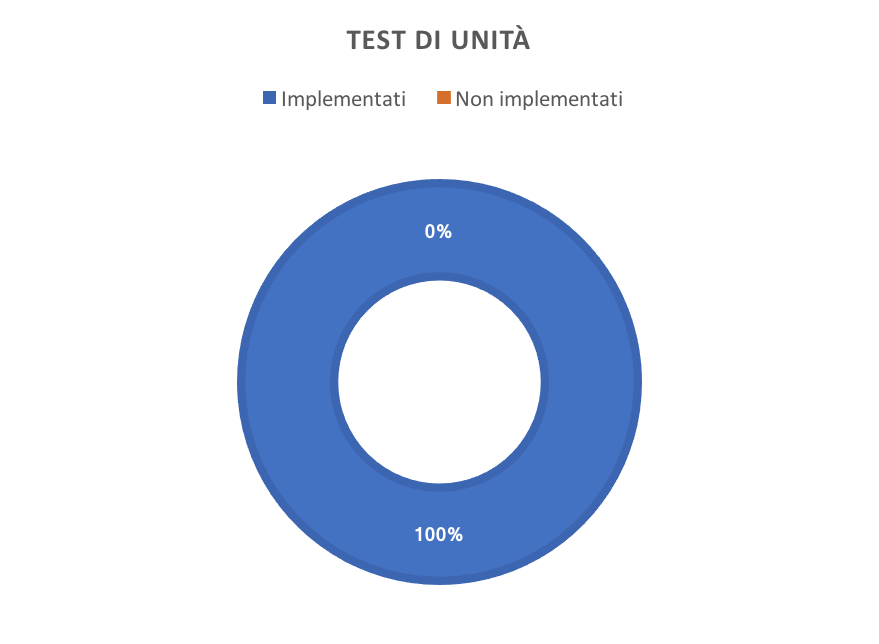
\includegraphics{ImgTest/TU.png}
			\caption{\textbf{Test di unità}: sommario grafico di completamento}
			\label{fig:pieTU}
		\end{figure}

	\newpage
	\subsection{Test di integrazione}
	I test di integrazione saranno descritti nel modo seguente:
	\begin{center}
		\textbf{TI[IdComponente]}
	\end{center}
	dove:
	\begin{itemize}
		\item \textbf{IdComponente} rappresenta il codice identificativo crescente del componente considerato.
	\end{itemize}
	È stato scelto di utilizzare un approccio top-down nel determinare i test di integrazione. Di seguito viene riportato un diagramma informale per rendere chiara la struttura dei test identificati.
	\\
	\begin{longtable}[c] { >{\centering\arraybackslash}p{4cm} p{7cm} >{\centering\arraybackslash}p{4cm}}
		\toprule
		\centerline{\textbf{ID test}} & \centerline{\textbf{Descrizione}} & \centerline{\textbf{Stato}} \\
			\midrule
			TI1 & Viene verificato che l'applicazione Web gestisca correttamente il Front-End del prodotto e le sue interazioni con il Back-End & Implementato \\
			\addlinespace[0.3em]
			\midrule
			\addlinespace[0.3em]
			TI2 & Viene verificato che i Service permettano di interagire correttamente con il Back-End & Implementato \\
			\addlinespace[0.3em]
			\midrule
			\addlinespace[0.3em]
			TI3 & Viene verificato che la View e il Controller del Front-End guest-home interagiscano tra di loro correttamente & Implementato \\
			\addlinespace[0.3em]
			\midrule
			\addlinespace[0.3em]
			TI4 & Viene verificato che la View e il Controller del Front-End amministrazione interagiscano tra di loro correttamente & Implementato \\
			\addlinespace[0.3em]
			\midrule
			\addlinespace[0.3em]
			TI5 & Viene verificato che il Model del Front-End guest-home e amministrazione rispecchi il rispettivo Controller & Implementato \\
			\addlinespace[0.3em]
			\midrule
			\addlinespace[0.3em]
			TI6 & Viene verificato che l'applicazione Web gestisca correttamente il Back-End del prodotto in modo tale da fornire al Front-End tutte le informazioni richieste & Implementato \\
			\addlinespace[0.3em]
			\midrule
			\addlinespace[0.3em]
			TI7 & Viene verificato che il Back-End si integri correttamente con le API Slack & Implementato \\
			\addlinespace[0.3em]
			\midrule
			\addlinespace[0.3em]
			TI8 & Viene verificato che il Back-End si integri correttamente con il database & Implementato \\
			\addlinespace[0.3em]
			\midrule
			\addlinespace[0.3em]
			TI9 & Viene verificato che i Service del Front-End amministrazione e guest-home riescano a chiamare le API dell'APIGateway correttamente & Implementato \\
			\addlinespace[0.3em]
			\midrule
			\addlinespace[0.3em]
			TI10 & Viene verificato che l'APIGateway chiami correttamente le function del Back-End & Implementato \\
			\addlinespace[0.3em]
			\midrule
			\addlinespace[0.3em]
			TI11 & Viene verificato che i Controller del front-end amminsitrazione si integrino correttamente con il rispettivo Service & Implementato \\
			\addlinespace[0.3em]
			\midrule
			\addlinespace[0.3em]
			TI12 & Viene verificato che i Controller del Front-End guest-home si integrino correttamente con il rispettivo Service & Implementato \\
			\addlinespace[0.3em]
			\midrule
			\addlinespace[0.3em]
			TI13 & Viene verificato che le chiamate di Interaction ad AVS siano corrette & Non implementato \\
			\addlinespace[0.3em]
			\midrule
			\addlinespace[0.3em]
			TI14 & Viene verificato che il Service del front-end si integri correttamente con il Controller dell'AmminisitrationView che lo richiama & Implementato \\
			\addlinespace[0.3em]
			\midrule
			\addlinespace[0.3em]
			TI15 & Viene verificato che il Service del Front-End si integri correttamente con il Controller del GuestComponents che lo richiama & Implementato \\
			\addlinespace[0.3em]
			\midrule
			\addlinespace[0.3em]
			TI16 & Viene verificato che i Controller gestiscano correttamente le \gl{root} di AngularJS & Implementato \\
			\addlinespace[0.3em]
			\midrule
			\addlinespace[0.3em]
			TI17 & Viene verificato che ManageAuth permetta di gestire l'autenticazione & Implementato \\
			\addlinespace[0.3em]
			\midrule
			\addlinespace[0.3em]
			TI18 & Viene verificato che ManageSlack permetta di gestire Slack & Implementato \\
			\addlinespace[0.3em]
			\midrule
			\addlinespace[0.3em]
			TI19 & Viene verificato che ManageQuestion permetta di gestire le domande & Implementato \\
			\addlinespace[0.3em]
			\midrule
			\addlinespace[0.3em]
			TI20 & Viene verificato che ManageAdmin permetta di gestire gli amministratori & Implementato \\
			\addlinespace[0.3em]
			\midrule
			\addlinespace[0.3em]
			TI21 & Viene verificato che ManageFirms permetta di gestire le aziende & Implementato \\
			\bottomrule
			\caption{Specifica test di integrazione}
	\end{longtable}

		\vspace*{1cm}
		\subsubsection{Grado di completamento dei test di integrazione}

		Di seguito è fornito, tramite un \textit{pie chart}, un sommario sul grado di completamento dei \textbf{test di integrazione} effettuati:

		\begin{figure}[!h]
			\centering
			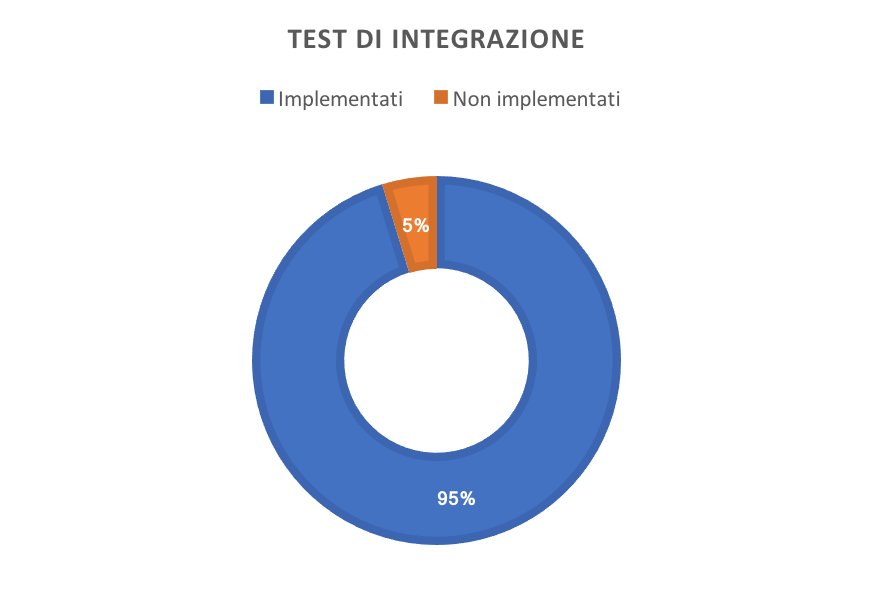
\includegraphics{ImgTest/TI.png}
			\caption{\textbf{Test di integrazione:} sommario grafico di completamento}
			\label{fig:pieTI}
		\end{figure}

	\newpage
	\newpage
	\subsection{Test di sistema}
	I test di sistema saranno descritti nel modo seguente:
	\begin{center}
		\textbf{TS[TipoRequisito][ImportanzaRequisito][IdRequisito]}
	\end{center}
	dove:
	\begin{itemize}
		\item \textbf{TipoRequisito} può assumere valori compresi tra:
		\begin{itemize}
			\item F per i requisiti funzionali;
			\item Q per i requisiti di qualità;
			\item V per i requisiti di vincolo;
			\item P per i requisiti prestazionali.
		\end{itemize}
		\item \textbf{ImportanzaRequisito} può assumere valori compresi tra:
		\begin{itemize}
			\item D per i requisiti desiderabili;
			\item O per i requisiti di obbligatori;
			\item F per i requisiti di facoltativi.
		\end{itemize}
		\item \textbf{IdRequisito} assume un valore gerarchico che identifica il singolo requisito.
	\end{itemize}

	\begin{longtable}[c] { >{\centering\arraybackslash}p{2cm} p{7cm} >{\centering\arraybackslash}p{4cm} >{\centering\arraybackslash}p{2cm}}
		\toprule
		\centerline{\textbf{ID test}} & \centerline{\textbf{Descrizione}} & \centerline{\textbf{Stato}} & \centerline{\textbf{Requisito}}\\
			\midrule
			TSFF1 & Viene verificato che l'utente possa attivare il sistema tramite comando vocale & Non implementato & RFF1 \\
			\addlinespace[0.3em]
			\midrule
			\addlinespace[0.3em]
			TSOF2 & L'utente deve poter attivare il sistema tramite pulsante & Implementato & ROF2 \\
			\addlinespace[0.3em]
			\midrule
			\addlinespace[0.3em]
			TSOF3 & Il sistema deve poter disattivarsi in automatico per timeout & Implementato & ROF3 \\
			\addlinespace[0.3em]
			\midrule
			\addlinespace[0.3em]
			TSOF4 & L'utente deve poter disattivare il sistema in qualsiasi momento tramite comando vocale & Non implementato & ROF4 \\
			\addlinespace[0.3em]
			\midrule
			\addlinespace[0.3em]
			TSOF5 & L'utente deve poter disattivare il sistema in qualsiasi momento tramite pulsante & Implementato & RFF5 \\
			\addlinespace[0.3em]
			\midrule
			\addlinespace[0.3em]
			TSOF6 & L'utente deve poter identificarsi nel sistema per usufruirne & Implementato & ROF6 \\
			\addlinespace[0.3em]
			\midrule
			\addlinespace[0.3em]
			TSOF7 & Il sistema deve poter chiedere all'ospite il proprio nome e cognome & Implementato & ROF7 \\
			\addlinespace[0.3em]
			\midrule
			\addlinespace[0.3em]
			TSOF8 & Il sistema deve rimanere in ascolto del nome e del cognome dell'ospite per un periodo di tempo prefissato & Implementato & ROF8 \\
			\addlinespace[0.3em]
			\midrule
			\addlinespace[0.3em]
			TSOF9 & L'utente deve poter rispondere vocalmente indicando il proprio nome e cognome & Implementato & ROF9 \\
			\addlinespace[0.3em]
			\midrule
			\addlinespace[0.3em]
			TSOF10 & L'utente deve poter confermare nome e cognome inseriti vocalmente & Non implementato & RFF10 \\
			\addlinespace[0.3em]
			\midrule
			\addlinespace[0.3em]
			TSOF11 & Un amministratore deve poter effettuare il login al sistema & Implementato & ROF11 \\
			\addlinespace[0.3em]
			\midrule
			\addlinespace[0.3em]
			TSOF12 & Un amministratore deve poter inserire la propria email per effettuare il login nel sistema & Implementato & ROF12 \\
			\addlinespace[0.3em]
			\midrule
			\addlinespace[0.3em]
			TSOF13 & Un amministratore deve poter confermare la propria email per effettuare il login nel sistema & Implementato & ROF13 \\
			\addlinespace[0.3em]
			\midrule
			\addlinespace[0.3em]
			TSOF14 & Un amministratore deve poter recuperare la propria password & Implementato & ROF14 \\
			\addlinespace[0.3em]
			\midrule
			\addlinespace[0.3em]
			TSOF15 & Un amministratore deve poter inserire la propria email per recuperare la propria password & Implementato & ROF15 \\
			\addlinespace[0.3em]
			\midrule
			\addlinespace[0.3em]
			TSOF16 & Un amministratore deve poter confermare la propria email per recuperare la propria password & Implementato & ROF16 \\
			\addlinespace[0.3em]
			\midrule
			\addlinespace[0.3em]
			TSOF17 & Un amministratore deve poter modificare la password inserita per effettuare il login nel sistema	& Implementato & ROF17 \\
			\addlinespace[0.3em]
			\midrule
			\addlinespace[0.3em]
			TSOF18 & Un amministratore deve poter confermare la password inserita per effettuare il login nel sistema & Implementato & ROF18 \\
			\addlinespace[0.3em]
			\midrule
			\addlinespace[0.3em]
			TSOF19 & La password deve essere alfanumerica e deve essere lunga almeno 8 caratteri & Implementato & ROF19 \\
			\addlinespace[0.3em]
			\midrule
			\addlinespace[0.3em]
			TSOF20 & Un amministratore deve poter visualizzare un messaggio di errore se la password inserita non è corretta & Implementato & ROF20 \\
			\addlinespace[0.3em]
			\midrule
			\addlinespace[0.3em]
			TSOF21 & Un amministratore deve poter visualizzare un messaggio di errore se la email inserita non è presente nel sistema & Implementato & ROF21 \\
			\addlinespace[0.3em]
			\midrule
			\addlinespace[0.3em]
			TSOF22 & L'ospite deve poter interagire con il sistema rispondendo alle domande che gli vengono poste & Implementato & ROF22 \\
			\addlinespace[0.3em]
			\midrule
			\addlinespace[0.3em]
			TSOF23 & L'ospite deve poter interagire con il sistema vocalmente & Implementato & ROF23 \\
			\addlinespace[0.3em]
			\midrule
			\addlinespace[0.3em]
			TSOF24 & Il sistema deve poter verificare se un ospite è già registrato o meno & Implementato & ROF24\\
			\addlinespace[0.3em]
			\midrule
			\addlinespace[0.3em]
			TSOF25 & l sistema deve poter adattare le domande in base al numero di presenze precedenti dell'ospite & Implementato & ROF25 \\
			\addlinespace[0.3em]
			\midrule
			\addlinespace[0.3em]
			TSOF26 & Il sistema deve poter chiedere all'ospite l'azienda di appartenenza & Implementato & ROF26 \\
			\addlinespace[0.3em]
			\midrule
			\addlinespace[0.3em]
			TSOF27 & Il sistema deve poter rimanere in ascolto, del nome dell'azienda dell'ospite, per un periodo di tempo prefissato & Implementato & ROF27 \\
			\addlinespace[0.3em]
			\midrule
			\addlinespace[0.3em]
			TSOF28 & L'utente deve poter confermare l'azienda inserita vocalmente & Implementato & ROF28 \\
			\addlinespace[0.3em]
			\midrule
			\addlinespace[0.3em]
			TSOF29 & Il sistema deve poter chiedere all'ospite l'interlocutore ricercato & Implementato & ROF29 \\
			\addlinespace[0.3em]
			\midrule
			\addlinespace[0.3em]
			TSOF30 & Il sistema deve poter rimanere in ascolto, del nome della persona cercata da parte dell'ospite, per un periodo di tempo prefissato & Implementato & ROF30 \\
			\addlinespace[0.3em]
			\midrule
			\addlinespace[0.3em]
			TSOF31 & L'utente deve poter confermare il nome dell’interlocutore inserito vocalmente & Implementato & ROF31 \\
			\addlinespace[0.3em]
			\midrule
			\addlinespace[0.3em]
			TSOF32 & Il sistema deve poter chiedere all'ospite se desidera un caffè & Implementato & ROF32 \\
			\addlinespace[0.3em]
			\midrule
			\addlinespace[0.3em]
			TSOF33 & Il sistema deve poter rimanere in ascolto di una risposta da parte dell'ospite per un periodo di tempo prefissato	 & Implementato & ROF33 \\
			\addlinespace[0.3em]
			\midrule
			\addlinespace[0.3em]
			TSOF34 & Il sistema deve poter chiedere all'ospite se necessita di qualche materiale & Implementato & ROF34 \\
			\addlinespace[0.3em]
			\midrule
			\addlinespace[0.3em]
			TSOF35 & Il sistema deve poter rimanere in ascolto di una risposta da parte dell'ospite per un periodo di tempo prefissato & Implementato & ROF35 \\
			\addlinespace[0.3em]
			\midrule
			\addlinespace[0.3em]
			TSOF36 & Il sistema deve poter intrattenere l'ospite con determinati argomenti & Implementato & ROF36 \\
			\addlinespace[0.3em]
			\midrule
			\addlinespace[0.3em]
			TSOF37 & Il sistema deve poter intrattenere l'ospite con il meteo di una località scelta & Non implementato & ROF37 \\
			\addlinespace[0.3em]
			\midrule
			\addlinespace[0.3em]
			TSOF38 & Il sistema deve poter intrattenere l'ospite con alcune news & Non implementato & ROF38 \\
			\addlinespace[0.3em]
			\midrule
			\addlinespace[0.3em]
			TSOF39 & Il sistema deve poter intrattenere l'ospite con alcune barzellette & Implementato & ROF39 \\
			\addlinespace[0.3em]
			\midrule
			\addlinespace[0.3em]
			TSOF40 & Il sistema deve poter visualizzare a schermo le possibili aziende di appartenenza & Non implementato & ROF40 \\
			\addlinespace[0.3em]
			\midrule
			\addlinespace[0.3em]
			TSOF41 & Un amministratore deve poter effettuare il logout dal sistema solo se loggato	 & Implementato & ROF41 \\
			\addlinespace[0.3em]
			\midrule
			\addlinespace[0.3em]
			TSOF42 & Il sistema deve poter essere gestito da un pannello di amministrazione & Implementato & ROF42 \\
			\addlinespace[0.3em]
			\midrule
			\addlinespace[0.3em]
			TSOF43 & L'Admin deve poter gestire gli ospiti & Implementato & ROF43 \\
			\addlinespace[0.3em]
			\midrule
			\addlinespace[0.3em]
			TSOF44 & L'Admin deve poter scegliere un ospite da rinominare & Non implementato & ROF44 \\
			\addlinespace[0.3em]
			\midrule
			\addlinespace[0.3em]
			TSOF45 & L'Admin deve poter rinominare un ospite & Non implementato & ROF45 \\
			\addlinespace[0.3em]
			\midrule
			\addlinespace[0.3em]
			TSOF46 & L'Admin deve poter confermare la rinomina di un ospite & Non implementato & ROF46 \\
			\addlinespace[0.3em]
			\midrule
			\addlinespace[0.3em]
			TSOF47 & L'Admin deve poter scegliere un'azienda da rinominare & Non implementato & ROF47 \\
			\addlinespace[0.3em]
			\midrule
			\addlinespace[0.3em]
			TSOF48 & L'Admin deve poter rinominare un'azienda & Non implementato & ROF48 \\
			\addlinespace[0.3em]
			\midrule
			\addlinespace[0.3em]
			TSOF49 & L'Admin deve poter confermare la rinomina di un'azienda & Non implementato & ROF49 \\
			\addlinespace[0.3em]
			\midrule
			\addlinespace[0.3em]
			TSOF50 & L'Admin deve poter visualizzare il profilo di un ospite & Implementato & ROF50 \\
			\addlinespace[0.3em]
			\midrule
			\addlinespace[0.3em]
			TSOF51 & L'Admin deve poter gestire le domande & Implementato & ROF51 \\
			\addlinespace[0.3em]
			\midrule
			\addlinespace[0.3em]
			TSOF52 & L'Admin deve poter aggiungere una domanda & Implementato & ROF52 \\
			\addlinespace[0.3em]
			\midrule
			\addlinespace[0.3em]
			TSOF53 & L'Admin deve poter confermare l'inserimento di una domanda & Implementato & ROF53 \\
			\addlinespace[0.3em]
			\midrule
			\addlinespace[0.3em]
			TSOF54 & L'Admin deve poter scegliere una domanda da rimuovere	& Implementato & ROF54 \\
			\addlinespace[0.3em]
			\midrule
			\addlinespace[0.3em]
			TSOF55 & L'Admin deve poter confermare la rimozione di una domanda & Implementato & ROF55 \\
			\addlinespace[0.3em]
			\midrule
			\addlinespace[0.3em]
			TSOF56 & L'Admin deve poter scegliere una domanda da modificare	 & Implementato & ROF56 \\
			\addlinespace[0.3em]
			\midrule
			\addlinespace[0.3em]
			TSOF57 & L'Admin deve poter confermare la modifica ad una domanda & Implementato & ROF57 \\
			\addlinespace[0.3em]
			\midrule
			\addlinespace[0.3em]
			TSOF58 & L'Admin deve poter gestire le risposte & Implementato & ROF58 \\
			\addlinespace[0.3em]
			\midrule
			\addlinespace[0.3em]
			TSOF59 & L'Admin deve poter aggiungere una risposta & Implementato & ROF59 \\
			\addlinespace[0.3em]
			\midrule
			\addlinespace[0.3em]
			TSOF60 & L'Admin deve poter confermare l'inserimento di una risposta & Implementato & ROF60 \\
			\addlinespace[0.3em]
			\midrule
			\addlinespace[0.3em]
			TSOF61 & L'Admin deve poter modificare una risposta & Non implementato & ROF61 \\
			\addlinespace[0.3em]
			\midrule
			\addlinespace[0.3em]
			TSOF62 & L'Admin deve poter confermare la modifica di una risposta & Non implementato & ROF62 \\
			\addlinespace[0.3em]
			\midrule
			\addlinespace[0.3em]
			TSOF63 & L'Admin deve poter scegliere una risposta da rimuovere & Implementato & ROF63 \\
			\addlinespace[0.3em]
			\midrule
			\addlinespace[0.3em]
			TSOF64 & L'Admin deve poter confermare la rimozione di una risposta & Implementato & ROF64 \\
			\addlinespace[0.3em]
			\midrule
			\addlinespace[0.3em]
			TSOF65 & L'Admin deve poter scegliere una ACTION da associare ad una risposta & Implementato & ROF65 \\
			\addlinespace[0.3em]
			\midrule
			\addlinespace[0.3em]
			TSOF66 & L'Admin deve poter modificare il testo di una risposta & Implementato & ROF66 \\
			\addlinespace[0.3em]
			\midrule
			\addlinespace[0.3em]
			TSOF67 & L'Admin deve poter inserire una risposta lunga almeno N caratteri, con N un numero predefinito dal sistema & Implementato & ROF67 \\
			\addlinespace[0.3em]
			\midrule
			\addlinespace[0.3em]
			TSOF68 & L'Admin deve poter inserire l'associazione con una domanda successiva & Implementato & ROF68 \\
			\addlinespace[0.3em]
			\midrule
			\addlinespace[0.3em]
			TSOF69 & L'Admin deve poter modificare l'associazione di una domanda successiva	 & Implementato & ROF69 \\
			\addlinespace[0.3em]
			\midrule
			\addlinespace[0.3em]
			TSOF70 & L'Admin deve poter modificare il testo di una domanda base & Implementato & ROF70 \\
			\addlinespace[0.3em]
			\midrule
			\addlinespace[0.3em]
			TSOF71 & L'Admin deve poter inserire una domanda base lunga almeno N caratteri, con N un numero predefinito dal sistema & Implementato & ROF71 \\
			\addlinespace[0.3em]
			\midrule
			\addlinespace[0.3em]
			TSOF72 & L'Admin deve poter modificare il testo di una domanda ricorrente & Implementato & ROF72 \\
			\addlinespace[0.3em]
			\midrule
			\addlinespace[0.3em]
			TSOF73 & L’Admin deve poter inserire una domanda ricorrente lunga almeno N caratteri, con N un numero predefinito dal sistema & Implementato & ROF73 \\
			\addlinespace[0.3em]
			\midrule
			\addlinespace[0.3em]
			TSOF74 & L'Admin deve poter gestire le impostazioni di Slack & Implementato & ROF74 \\
			\addlinespace[0.3em]
			\midrule
			\addlinespace[0.3em]
			TSOF75 & L'Admin deve poter gestire una lista di interlocutori di default per i canali \#azienda che vengono creati & Implementato & ROF75 \\
			\addlinespace[0.3em]
			\midrule
			\addlinespace[0.3em]
			TSOF76 & L'Admin deve poter scegliere un interlocutore da associare alla lista di default	& Implementato & ROF76 \\
			\addlinespace[0.3em]
			\midrule
			\addlinespace[0.3em]
			TSOF77 & L'Admin deve poter confermare un interlocutore da associare alla lista di default	& Implementato & ROF77 \\
			\addlinespace[0.3em]
			\midrule
			\addlinespace[0.3em]
			TSOF78 & L'Admin deve poter scegliere un interlocutore da disassociare dalla lista di default & Implementato & ROF78 \\
			\addlinespace[0.3em]
			\midrule
			\addlinespace[0.3em]
			TSOF79 & L'Admin deve poter confermare un interlocutore da disassociare dalla lista di default & Implementato & ROF79 \\
			\addlinespace[0.3em]
			\midrule
			\addlinespace[0.3em]
			TSOF80 & L'Admin deve poter aggiornare la lista di interlocutori & Implementato & ROF80 \\
			\addlinespace[0.3em]
			\midrule
			\addlinespace[0.3em]
			TSOF81 & L'Admin deve poter gestire il proprio account & Implementato & ROF81 \\
			\addlinespace[0.3em]
			\midrule
			\addlinespace[0.3em]
			TSOF82 & L'Admin deve poter modificare la propria password di accesso & Implementato & ROF82 \\
			\addlinespace[0.3em]
			\midrule
			\addlinespace[0.3em]
			TSOF83 & L'Admin deve poter inserire una nuova password di accesso (alfanumerica e di almeno 8 caratteri) & Implementato & ROF83 \\
			\addlinespace[0.3em]
			\midrule
			\addlinespace[0.3em]
			TSOF84 & L'Admin deve poter confermare la modifica della password di accesso & Implementato & ROF84 \\
			\addlinespace[0.3em]
			\midrule
			\addlinespace[0.3em]
			TSOF85 & Il Super Admin deve poter aver accesso a tutte le funzionalità di un normale Admin & Implementato & ROF85 \\
			\addlinespace[0.3em]
			\midrule
			\addlinespace[0.3em]
			TSOF86 & Il Super Admin deve poter modificare le email di accesso di un qualsiasi Admin	& Implementato & ROF86 \\
			\addlinespace[0.3em]
			\midrule
			\addlinespace[0.3em]
			TSOF87 & Il Super Admin deve poter confermare la modifica della email di accesso di un qualsiasi Admin & Implementato & ROF87 \\
			\addlinespace[0.3em]
			\midrule
			\addlinespace[0.3em]
			TSOF88 & Il Super Admin deve poter modificare le password di accesso di un qualsiasi Admin & Implementato & ROF88 \\
			\addlinespace[0.3em]
			\midrule
			\addlinespace[0.3em]
			TSOF89 & Il Super Admin deve poter confermare la modifica della password di accesso di un qualsiasi Admin & Implementato & ROF89 \\
			\addlinespace[0.3em]
			\midrule
			\addlinespace[0.3em]
			TSOF90 & Il Super Admin non deve poter visualizzare la password di accesso di un qualsiasi Admin & Implementato & ROF90 \\
			\addlinespace[0.3em]
			\midrule
			\addlinespace[0.3em]
			TSOF91 & Il Super Admin deve poter aggiungere un nuovo Admin al sistema	 & Implementato & ROF91 \\
			\addlinespace[0.3em]
			\midrule
			\addlinespace[0.3em]
			TSOF92 & Il Super Admin deve poter confermare l'aggiunta un nuovo Admin al sistema & Implementato & ROF92 \\
			\addlinespace[0.3em]
			\midrule
			\addlinespace[0.3em]
			TSOF93 & Il Super Admin deve poter rimuovere un qualsiasi Admin dal sistema	 & Implementato & ROF93 \\
			\addlinespace[0.3em]
			\midrule
			\addlinespace[0.3em]
			TSOF94 & Il Super Admin deve poter confermare la rimozione di un qualsiasi Admin dal sistema & Implementato & ROF94 \\
		\bottomrule
		\caption{Specifica test di sistema}
	\end{longtable}

	\newpage
		\subsubsection{Grado di completamento dei test di sistema}

		Di seguito è fornito, tramite un \textit{pie chart}, un sommario sul grado di completamento dei \textbf{test di sistema} effettuati:

		\begin{figure}[!h]
			\centering
			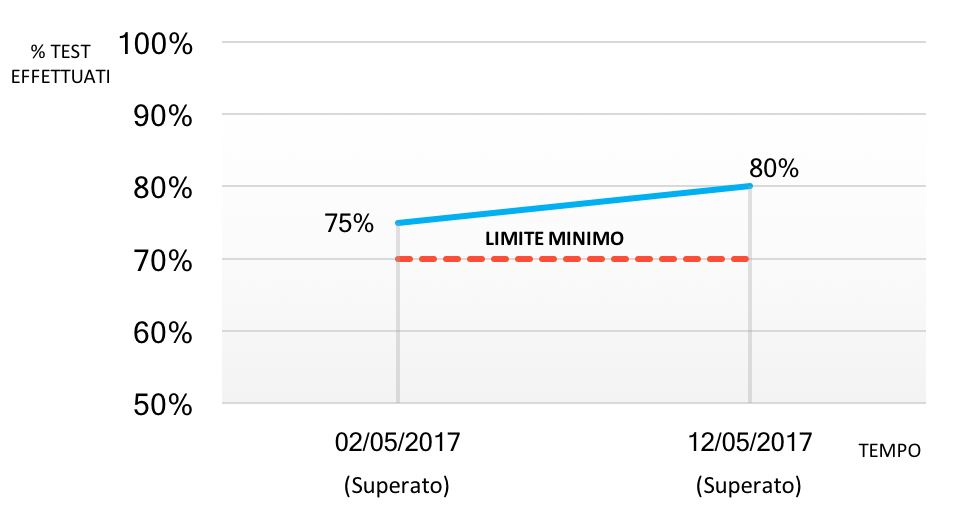
\includegraphics{ImgTest/TS.png}
			\caption{\textbf{Test di sistema}: sommario grafico di completamento}
			\label{fig:pieTS}
		\end{figure}

	\newpage
	\subsection{Test di non regressione}
	I test di non regressione saranno descritti nel modo seguente:
	\begin{center}
		\textbf{TNR[IdComponente]}
	\end{center}
	dove:
	\begin{itemize}
		\item \textbf{IdComponente} rappresenta il codice identificativo crescente del componente considerato.
	\end{itemize}
	Di seguito viene riportato un diagramma informale per rendere chiara la struttura dei test identificati.
	\\
	\begin{longtable}[c] { >{\centering\arraybackslash}p{4cm} p{7cm} >{\centering\arraybackslash}p{4cm}}
		\toprule
		\centerline{\textbf{ID test}} & \centerline{\textbf{Descrizione}} & \centerline{\textbf{Stato}} \\
			\midrule
			TNR1 & Viene verificato che ManageAuth permetta delle modifiche mantenendo le sue funzionalità & Implementato \\
			\addlinespace[0.3em]
			\midrule
			\addlinespace[0.3em]
			TNR2 & Viene verificato che ManageSlack permetta delle modifiche mantenendo le sue funzionalità & Implementato \\
			\addlinespace[0.3em]
			\midrule
			\addlinespace[0.3em]
			TNR3 & Viene verificato che ManageQuestion permetta delle modifiche mantenendo le sue funzionalità & Implementato \\
			\addlinespace[0.3em]
			\midrule
			\addlinespace[0.3em]
			TNR4 & Viene verificato che ManageAdmin permetta delle modifiche mantenendo le sue funzionalità & Implementato \\
			\addlinespace[0.3em]
			\midrule
			\addlinespace[0.3em]
			TNR5 & Viene verificato che ManageFirms permetta delle modifiche mantenendo le sue funzionalità & Implementato \\
			\bottomrule
			\caption{Specifica test di non regressione}
	\end{longtable}

	\newpage
	\subsubsection{Grado di completamento dei test di non regressione}

		Di seguito è fornito, tramite un \textit{pie chart}, un sommario sul grado di completamento dei \textbf{test di non regressione} effettuati:

		\begin{figure}[!h]
			\centering
			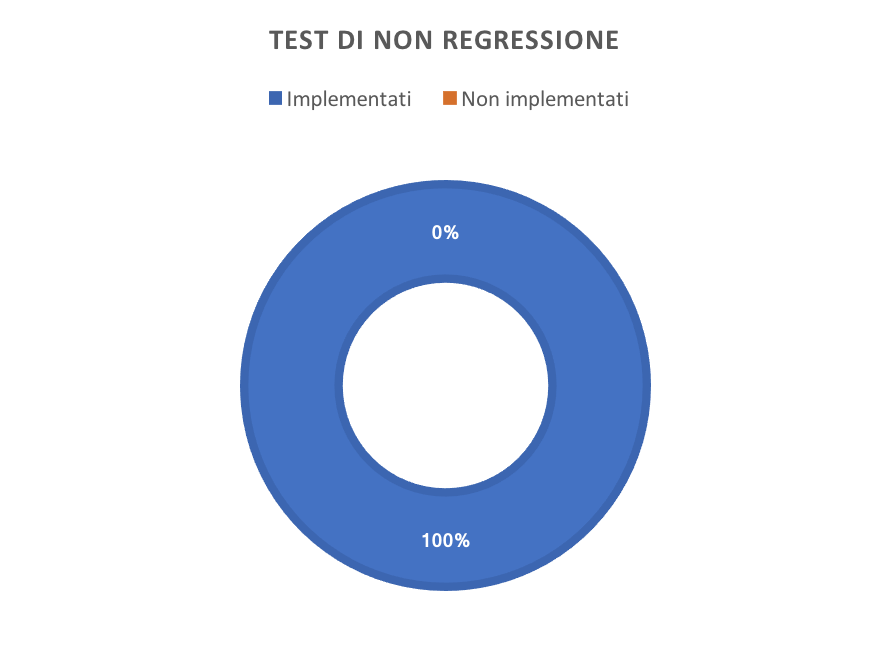
\includegraphics{ImgTest/TNR.png}
			\caption{Test di non regressione: sommario grafico di completamento}
			\label{fig:pieTNR}
		\end{figure}


	\newpage
	\subsection{Test di validazione}
	I test di validazione saranno organizzati nel modo seguente:
	\begin{center}
		\textbf{TV[IdRequisito]}
	\end{center}
	dove:	
	\textbf{IdRequisito} assume un valore gerarchico che identifica il singolo requisito.

	% INTRODUZIONE TODO

	\begin{longtable}[c] { >{\centering\arraybackslash}p{4cm} p{7cm} >{\centering\arraybackslash}p{4cm}}
		\toprule
		\centerline{\textbf{ID test}} & \centerline{\textbf{Descrizione}} & \centerline{\textbf{Esito}} \\
			\midrule
			TV1 & Il sistema deve poter chiedere all'ospite il proprio nome e cognome & Superato \\
			\addlinespace[0.3em]
			\midrule
			\addlinespace[0.3em]
			TV2 & Il sistema deve poter verificare se un ospite è già registrato o meno & Superato \\
			\addlinespace[0.3em]
			\midrule
			\addlinespace[0.3em]
			TV3 & Il sistema deve poter chiedere all'ospite l'azienda di appartenenza & Superato \\
			\addlinespace[0.3em]
			\midrule
			\addlinespace[0.3em]
			TV4 & Il sistema deve creare un canale Slack se la risposta alla domanda che richiede il nome dell'azienda appartenente è diverso da ``no`` & Superato \\
			\addlinespace[0.3em]
			\midrule
			\addlinespace[0.3em]
			TV5 &  Il sistema invia su Slack un avviso di arrivo ospite nel canale \#general quando quest'ultimo non appartiene ad una azienda & Superato \\
			\addlinespace[0.3em]
			\midrule
			\addlinespace[0.3em]
			TV6 &  Il sistema invia su Slack un avviso di arrivo ospite nel canale \#nomeAzienda quando quest'ultimo appartiene ad una azienda & Superato \\
			\addlinespace[0.3em]
			\midrule
			\addlinespace[0.3em]
			TV7 &  Il sistema deve poter chiedere all'ospite l'interlocutore ricercato & Superato \\
			\addlinespace[0.3em]
			\midrule
			\addlinespace[0.3em]
			TV8 &  Il sistema scrive su Slack l’interlocutore che l’ospite vuole incontrare & Superato \\
			\addlinespace[0.3em]
			\midrule
			\addlinespace[0.3em]
			TV9 &  Il sistema deve poter chiedere all'ospite se desidera un caffè & Superato \\
			\addlinespace[0.3em]
			\midrule
			\addlinespace[0.3em]
			TV10 & Il sistema scrive su Slack la conferma che l'ospite desidera un caffè & Superato \\
			\addlinespace[0.3em]
			\midrule
			\addlinespace[0.3em]
			TV11 & Il sistema ripete la domanda se non comprende correttamente la risposta.
			Questo per domande che richiedono una risposta della tipologia “yes” o “no” & Superato \\
			\addlinespace[0.3em]
			\midrule
			\addlinespace[0.3em]
			TV12 & Un amministratore deve poter aggiungere una domanda & Superato \\
			\addlinespace[0.3em]
			\midrule
			\addlinespace[0.3em]
			TV13 & Il sistema deve chiedere all'ospite se desidera essere intrattenuto & Superato \\
			\addlinespace[0.3em]
			\midrule
			\addlinespace[0.3em]
			TV14 & Il sistema deve poter intrattenere l'ospite con alcune barzellette & Superato \\
			\addlinespace[0.3em]
			\midrule
			\addlinespace[0.3em]
			TV15 & Il sistema deve poter permettere agli amministratori di rimuovere una domanda & Superato \\
			\addlinespace[0.3em]
			\midrule
			\addlinespace[0.3em]
			TV16 & Un amministratore deve poter aggiungere un interlocutore alla lista di default & Superato \\
			\addlinespace[0.3em]
			\midrule
			\addlinespace[0.3em]
			TV17 & Un amministratore deve poter rimuovere un interlocutore dalla lista di default & Superato \\
			\addlinespace[0.3em]
			\midrule
			\addlinespace[0.3em]
			TV18 & Un amministratore deve poter aggiungere una risposta & Superato \\
			\addlinespace[0.3em]
			\midrule
			\addlinespace[0.3em]
			TV19 & Un amministratore deve poter rimuovere una risposta & Superato \\
			\addlinespace[0.3em]
			\midrule
			\addlinespace[0.3em]
			TV20 & Un amministratore deve poter scegliere una ACTION da associare ad una risposta & Superato \\
			\addlinespace[0.3em]
			\midrule
			\addlinespace[0.3em]
			TV21 & Il sistema deve permettere agli amministratori di associare una \textit{questionAction} ad una \textit{question} & Superato \\
			\addlinespace[0.3em]
			\midrule
			\addlinespace[0.3em]
			TV22 & Il sistema deve permettere agli amministratori di disassociare una \textit{action} da una \textit{answer} & Superato \\
			\addlinespace[0.3em]
			\midrule
			\addlinespace[0.3em]
			TV23 & Il sistema deve permettere agli amministratori di disassociare una \textit{questionAction} da una \textit{question} & Superato \\
			\addlinespace[0.3em]
			\midrule
			\addlinespace[0.3em]
			TV24 & Un amministratore deve poter visualizzare a schermo la lista delle possibili aziende di appartenenza di un ospite & Superato \\
			\addlinespace[0.3em]
			\midrule
			\addlinespace[0.3em]
			TV25 & Un amministratore deve poter visualizzare il profilo di un ospite & Superato \\
			\addlinespace[0.3em]
			\midrule
			\addlinespace[0.3em]
			TV26 & Un amministratore deve poter effettuare il login nel sistema & Superato \\
			\addlinespace[0.3em]
			\midrule
			\addlinespace[0.3em]
			TV27 & Un amministratore deve poter effettuare il logout dal sistema & Superato \\
			\addlinespace[0.3em]
			\midrule
			\addlinespace[0.3em]
			TV28 & Un amministratore deve poter recuperare la propria password tramite l'apposita pagina & Superato \\
			\addlinespace[0.3em]
			\midrule
			\addlinespace[0.3em]
			TV29 & Il sistema deve scrivere i log della conversazione nella tabella \textit{guest\_interaction} del Database & Superato \\
			\bottomrule
			\caption{Specifica test di validazione}
	\end{longtable}


\end{document}
